\documentclass[10pt]{article}
\usepackage{icmlko}

\icmlmeta{IP 파운데이션 월드모델}{15}{DLC는 결과였다}{반증 조건 하나가 누출을 드러내고 노트 14를 철회시켰다 --- 그리고 노트 13은 살아남았다}

\begin{document}

\twocolumn[
\icmlheader

\begin{abstract}
노트 13은 게임 도메인이 대상으로서 어려운 이유를 라벨 성질로 돌리고 반증 조건을
적었다 --- 출시 후 30일 리뷰만 라벨로 쓰면 설명력이 올라야 하며, 오르지 않으면
문제는 라벨이 아니라 축 매핑이다. 434건에 대해 30일 창 라벨을 수집해 재봤다.
\textbf{오르지 않았다. 오히려 나빠졌다} --- 도메인 내부 모델조차 상수와 같아졌다
(0.8010 대 0.8004). 축 매핑을 추적하니 누출이 나왔다. Steam이 주는 DLC 목록은
\emph{현재} DLC이지 출시 시점 DLC가 아니다. 출시 1년 미만 게임의 평균 DLC는
3.09종이고 6년 이상은 18.47종이다. \textbf{성공한 게임이 DLC를 더 낸다 --- 역인과다.}
전체 리뷰와의 상관 $+$0.180이 30일 창 리뷰와는 $+$0.084로 반토막 난다. 이 축을
비우고 다시 쟀다. 결과가 갈린다. \textbf{노트 13은 살아남는다} --- 여섯 방향 중
넷이 여전히 유의하고, 게임이 낀 유의한 두 방향은 타깃 폭 하나만으로도 p$<$0.0001이다.
\textbf{노트 14는 철회한다} --- 공유 슬롯이 하나로 줄자 세 도메인 공동 학습이
어디서도 유의하지 않다(p=0.085, 0.520, 0.215). 부수적으로 노트 14의 정규화 버그도
찾아 고쳤다.
\end{abstract}
]

\section{반증 조건을 실행했다}

노트 13의 마지막 주장 상자는 이랬다.

\begin{quote}\fontsize{9.2}{11}\selectfont
게임 도메인이 대상으로서 어려운 것은 표본 크기가 아니라 라벨의 성질 때문이다.
리뷰 총계는 출시 시점 조건이 아니라 출시 이후 수년의 누적 동역학을 반영한다.\\[0.3em]
\textbf{반증 조건.} 출시 후 첫 30일 리뷰 수만 라벨로 쓰면 출시 시점 축의 설명력이
올라가야 한다. 오르지 않으면 라벨 성질이 아니라 축 매핑이 문제다.
\end{quote}

Steam 리뷰 API는 날짜 창을 받는다. 482건 중 창이 이미 닫힌 434건에 대해 출시 후
30일 안에 달린 리뷰 수를 수집했다. 창 라벨은 전체의 중앙 21.2\%다.

\begin{table}[t]
\centering\tsize
\caption{게임 라벨 정의별 성적(n=434). 낮을수록 좋다.}
\begin{tabular}{lrrr}
\toprule
라벨 & 상수 & 도메인 내부 & 평균 쌍 전이 \\
\midrule
전체 리뷰 & 0.7793 & 0.7649 & $+$0.0078 \\
출시 30일 리뷰 & 0.8004 & \textbf{0.8010} & $+$0.0404 \\
\bottomrule
\end{tabular}
\end{table}

\begin{figure}[t]
\centering
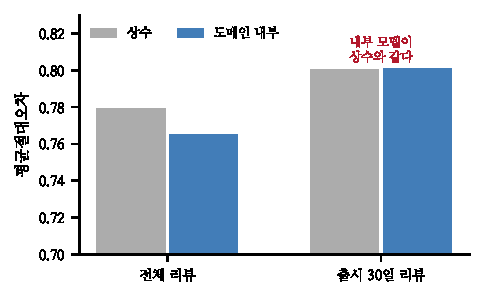
\includegraphics[width=\columnwidth]{figs/label.pdf}
\caption{30일 창으로 바꾸면 도메인 내부 모델조차 상수와 같아진다. 축이 출시
시점 반응에 대해 아무것도 말하지 못한다는 뜻이다.}
\end{figure}

올라가지 않았다. 그리고 더 나쁜 것은 \emph{도메인 내부} 성적이다. 게임 라벨을
전부 보고 적합한 모델이 상수와 같다(0.8010 대 0.8004). 축이 출시 시점 반응에
대해 아무 정보도 담고 있지 않다.

반증 조건이 말한 대로 문제는 라벨이 아니라 축 매핑이다.

\section{누출을 찾았다}

두 축 중 굿즈 규모를 의심했다. 게임에서 그것은 DLC 수였다.

\begin{figure}[t]
\centering
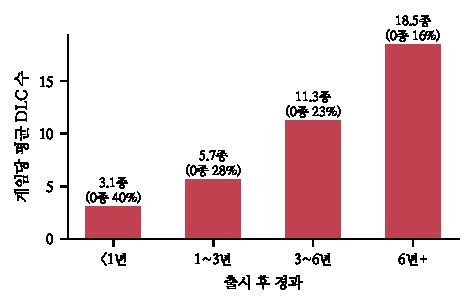
\includegraphics[width=\columnwidth]{figs/leak.pdf}
\caption{DLC 수는 출시 후 계속 늘어난다. 출시 시점 피처가 아니다.}
\end{figure}

\begin{table}[t]
\centering\tsize
\caption{출시 경과별 DLC 수(n=482).}
\begin{tabular}{lrrr}
\toprule
출시 후 & n & 평균 DLC & 0종 비율 \\
\midrule
1년 미만 & 173 & 3.09 & 40\% \\
1--3년 & 127 & 5.69 & 28\% \\
3--6년 & 90 & 11.27 & 23\% \\
6년 이상 & 92 & 18.47 & 16\% \\
\bottomrule
\end{tabular}
\end{table}

Steam \texttt{appdetails}의 \texttt{dlc} 목록은 조회 시점의 \emph{현재} DLC다.
출시 시점 DLC가 아니다. 6년 이상 된 게임의 평균 DLC가 1년 미만 게임의 6.0배다.

이것은 두 겹의 문제다.

\begin{itemize}[leftmargin=1.1em,itemsep=0.15em]
\item \textbf{시간 누적} --- 오래된 게임일수록 DLC가 많다. 탈추세로 상당 부분
      제거되지만 완전하지 않다.
\item \textbf{역인과} --- 성공한 게임이 DLC를 더 낸다. 이쪽이 본질이다.
      전체 리뷰와의 상관 $+$0.180이 30일 창 리뷰와는 $+$0.084로 반토막 난다.
      출시 시점 반응과는 관계가 약하고 \emph{누적 성공}과 관계가 강하다.
\end{itemize}

팝업에서 결과보고서의 일별 표로 운영일수를 세면 누출이라고 했던 것과 같은
구조다. 다른 점은 여기서는 내가 그것을 알아채지 못한 채 세 노트를 썼다는 것이다.

\claimx{게임 도메인의 굿즈 규모 축(DLC 수)은 누출이다. 출시 시점 조건이 아니라
출시 후 누적된 사후 정보이며, 그 상당 부분이 반응의 결과다.}{출시 시점
에디션 수(디럭스·컬렉터)를 따로 수집해 같은 자리에 넣었을 때 30일 창 라벨에
대한 설명력이 생기면, 문제는 '굿즈 규모'라는 축이 아니라 그 측정 방법이었다.}

\paragraph{팝업과 아이돌은 누출이 아니다}
팝업의 굿즈 종류 수는 기획서에 적히고, 아이돌의 앨범 버전 수는 발매 시점에
확정된다. 둘 다 출시 시점 피처다. 누출은 게임 도메인에 국한된다.

\section{그래서 무엇이 남았나}

게임의 굿즈 규모를 비우고 전부 다시 쟀다. 굿즈 규모가 유효한 팝업--아이돌 사이는
두 축으로, 게임이 낀 방향은 타깃 폭 하나로 검정한다.

\begin{figure}[t]
\centering
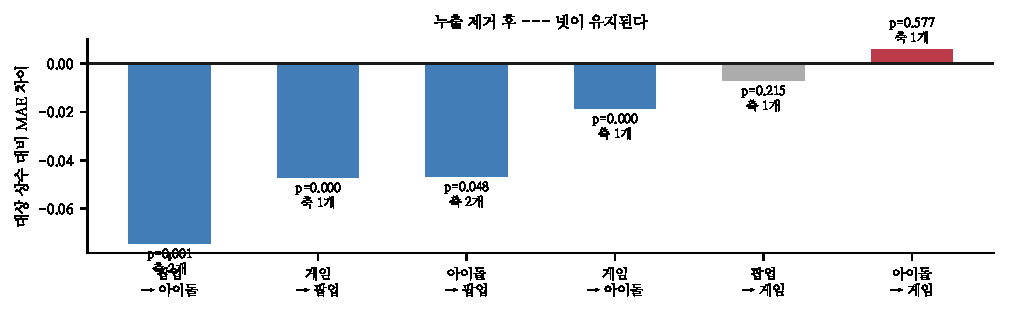
\includegraphics[width=\textwidth]{figs/retract.pdf}
\caption{누출 제거 후 여섯 방향. 넷이 유의하게 남는다.}
\end{figure}

\begin{table}[t]
\centering\tsize
\caption{누출 제거 후 전이. 순열 3,000회.}
\begin{tabular}{lrrrl}
\toprule
방향 & 축 & n & 차이 & p \\
\midrule
팝업 $\to$ 아이돌 & 2 & 63 & $-$0.0744 & \textbf{0.0013} \\
게임 $\to$ 팝업 & 1 & 75 & $-$0.0470 & \textbf{$<$0.0001} \\
아이돌 $\to$ 팝업 & 2 & 75 & $-$0.0467 & \textbf{0.0480} \\
게임 $\to$ 아이돌 & 1 & 74 & $-$0.0185 & \textbf{$<$0.0001} \\
팝업 $\to$ 게임 & 1 & 482 & $-$0.0069 & 0.2147 \\
아이돌 $\to$ 게임 & 1 & 482 & $+$0.0059 & 0.5770 \\
\bottomrule
\end{tabular}
\end{table}

\textbf{노트 13은 살아남는다.} 여섯 방향 중 넷이 여전히 유의하고, 게임이 낀
유의한 두 방향은 \emph{타깃 폭 하나만으로} p$<$0.0001이다. 그 방향들이 작동한
이유는 누출된 축 때문이 아니었다.

계수 부호도 유지된다 --- 타깃 폭은 팝업 $+$0.335, 아이돌 $+$0.441, 게임 $+$0.187로
세 도메인 모두 양수다.

\section{그러나 노트 14는 철회한다}

파운데이션 모델은 사정이 다르다. 공유 슬롯이 둘에서 하나로 줄었기 때문이다.

\begin{table}[t]
\centering\tsize
\caption{도메인 하나 빼기, 슬롯 1개(타깃 폭)로 재실행.}
\begin{tabular}{lrrrl}
\toprule
대상 & 상수 & 파운데이션 & 차이 & p \\
\midrule
팝업   & 0.7596 & 0.7239 & $-$0.0357 & 0.085 \\
아이돌 & 0.6588 & 0.6622 & $+$0.0034 & 0.520 \\
게임   & 0.7701 & 0.7630 & $-$0.0072 & 0.215 \\
\bottomrule
\end{tabular}
\end{table}

셋 다 유의하지 않다. 노트 14가 보고한 성공은 게임을 출처로 쓸 때 그 도메인의
누출된 굿즈 축이 헤드에 실려 있었기 때문이다.

\claimx{노트 14의 ``두 도메인으로 학습한 공유 헤드가 세 번째 도메인의 라벨 없이
상수를 이긴다''를 철회한다. 누출을 제거하면 세 도메인 공동 학습은 어디서도
유의하지 않다.}{출시 시점 에디션 수를 수집해 공유 슬롯이 다시 둘이 됐을 때
유의성이 돌아오면, 철회 사유는 누출이 아니라 슬롯 개수였던 것이다.}

\subsection{왜 쌍 전이는 되는데 공동 학습은 안 되나}

계수 크기가 도메인마다 다르기 때문으로 보인다. 타깃 폭 계수가 팝업 $+$0.335,
아이돌 $+$0.441, 게임 $+$0.187로 2.4배 차이가 난다. 공유 헤드는 하나의 기울기를
써야 하므로 세 값의 절충으로 끌려간다. 슬롯이 여럿이면 다른 슬롯이 보정할 여지가
있지만 하나면 그럴 수 없다.

\claimx{공유 헤드가 작동하려면 계수의 부호만 같아서는 부족하고 크기도 비슷해야
한다. 슬롯이 하나일 때 이 제약이 가장 세다.}{도메인별 스케일 항을 하나 더 두어
(공유 기울기 $\times$ 도메인 배율) 유의성이 돌아오면, 문제는 부호가 아니라
눈금이었던 것이다.}

\section{부수 발견 --- 노트 14의 정규화 버그}

노트 14를 쓰면서 앵커 타깃을 도메인마다 min-max로 0--1에 맞췄다. min-max는
극단값이 눈금을 정하므로 도메인 사이의 축 눈금이 어긋난다. 실제로 아이돌 $\to$
팝업 전이가 노트 13의 $-$0.0467에서 $-$0.0064로 무너져 있었다.

모든 도메인에 \emph{같은 함수}(로지스틱)를 쓰도록 고치자 $-$0.0642로 돌아왔다.
비교 가능한 눈금을 만들려면 도메인별 통계가 아니라 공통 변환을 써야 한다.

\section{한계}

\begin{itemize}[leftmargin=1.1em,itemsep=0.15em]
\item 게임의 출시 시점 에디션 수를 아직 수집하지 못했다. 굿즈 규모 축이 게임에서
      정말 작동하는지는 미결이다.
\item 30일 창 라벨은 48건(창이 안 닫힌 최신작)을 제외했다. 최신 편향이 남는다.
\item 팝업·아이돌의 굿즈 규모가 누출이 아니라는 것은 논증이지 검정이 아니다.
      같은 30일 창 방식의 검정을 두 도메인에서도 해야 한다.
\item 계수 크기 차이가 공동 학습 실패의 원인이라는 설명은 아직 검정하지 않았다.
\end{itemize}

\section{다음}

\begin{enumerate}[leftmargin=1.3em,itemsep=0.15em]
\item 게임 출시 시점 에디션 수 수집 --- 공유 슬롯을 둘로 되돌린다.
\item 도메인별 배율 항을 둔 공유 헤드 --- 계수 크기 가설의 직접 검정.
\item 팝업·아이돌 굿즈 축의 누출 검정 --- 논증을 검정으로 바꾼다.
\item 다른 축들의 누출 점검 --- 미디어 투입(퍼블리셔 사전 실적)은 시간 인과적으로
      계산했으나 같은 종류의 문제가 없는지 확인.
\end{enumerate}

\vspace{0.6em}
\hrule height 0.3pt
\vspace{0.5em}
{\footnotesize
\textbf{참고문헌}\\[0.3em]
Kaufman, S., Rosset, S., Perlich, C. (2012). Leakage in data mining: formulation,
detection, and avoidance. \emph{ACM TKDD}, 6(4), 1--21.\\[0.15em]
Good, P. (2005). \emph{Permutation, Parametric, and Bootstrap Tests of Hypotheses},
3rd ed. Springer.\\[0.15em]
Standley, T. et al. (2020). Which tasks should be learned together in multi-task
learning? \emph{ICML 2020}, 9120--9132.\\[0.15em]
Ben-David, S. et al. (2010). A theory of learning from different domains.
\emph{Machine Learning}, 79(1--2), 151--175.
}

\end{document}
